\documentclass[12pt]{article}

\input{.house-style/preamble.tex}
\usepackage{float}
\usepackage{tikz}
\usetikzlibrary{arrows.meta}

\tikzset{
  ttpbox/.style={draw, rounded corners=2pt, align=center, inner sep=4pt,
                 minimum height=7.5mm, font=\small},
  ttpar/.style={-{Stealth[length=2mm]}, thick},
}

\fancyhead[L]{\small\scshape Online Resource 1: Proposed Empirical Designs}

\renewcommand{\thefigure}{S\arabic{figure}}

\hypersetup{
  pdftitle={Online Resource 1: Proposed Empirical Designs},
  pdfkeywords={large language models; corrective control; empirical design; projectibility},
}
\ifdefined\TTPANONYMOUS
  \hypersetup{pdfauthor={}}
\fi

\title{Online Resource 1:\\ Proposed Empirical Designs\\[0.5ex]
\large Supplement to \textit{Grounding Without Corrective Control:\\
Truth-Tracking Profiles for Large Language Models}}
\ifdefined\TTPANONYMOUS
\author{}
\date{}
\else
\author{Brett Reynolds\\
Humber Polytechnic \& University of Toronto\\
\href{mailto:brett.reynolds@humber.ca}{brett.reynolds@humber.ca}}
\date{14th August 2026}
\fi

\begin{document}
\maketitle

\noindent\textbf{Journal:} \textit{Synthese}

\section{Purpose}

This resource specifies three component tests proposed in the accompanying article: a
crossed route-by-task design, a comparison that varies checking-route independence, and a
temporal test of live answerability. The designs don't jointly distinguish the decomposition
from an unrestricted effective-coverage description. Their purpose is to test whether a
decomposition fixed before the outcomes are observed supports selective transfer,
diagnosis, and intervention. No empirical results are reported; the numerical results below
come only from constructed data.

Table~\ref{tab:rivals} states the inferential role of each design. It treats the tests as
validation arguments: an observed contrast supports a specified component only under the
declared architectural boundary, auxiliary assumptions, and manipulation checks. None is a
crucial experiment against every informational redescription.

\begin{table}[!t]
\centering
\small
\begin{tabular}{@{}>{\raggedright\arraybackslash}p{0.17\linewidth}>{\raggedright\arraybackslash}p{0.25\linewidth}>{\raggedright\arraybackslash}p{0.25\linewidth}>{\raggedright\arraybackslash}p{0.24\linewidth}@{}}
\toprule
Test & Decomposition & Strongest coverage reply & Evidential role \\
\midrule
Route by task & A supplied route should help most where the task requires it. & Conditional or effective coverage predicts the same pattern by distinguishing kinds of task-relevant information. & Tests the proposed route carving and selective transfer, not uniqueness. \\
Checker relation & Lower conditional error overlap should improve repair when marginal accuracy and baseline inputs are matched. & Conditional coverage predicts the advantage by representing information added given generator error. & Tests checking-route independence; distinguishes only a fixed input-coverage comparator. \\
Temporal update & A live route should transmit a source update that a frozen record can't. & Dynamic coverage predicts the same result because follow-up information differs. & Operationalizes live answerability; doesn't discriminate against dynamic coverage. \\
\bottomrule
\end{tabular}
\caption{Predictions and limits of the three component tests.}
\label{tab:rivals}
\end{table}

\section{Fake-data stress tests of the decomposition}

Constructed data can audit a proposed model comparison before it is used on real systems
\citep{gelman2020bayesianworkflow}. Their causal structure is chosen, so they cannot show
that the decomposition is true. The exercise asks whether the analysis can recover a known
architectural advantage, whether a simpler prespecified model can beat it, and whether
predictive gains improve intervention choice.

Let $p_0$ be an arrangement's probability of an initially correct answer. For a correction
opportunity, let $x$, $d$, and $i$ represent target access, detectability, and checking-route
independence as operationalized by task-specific conditional non-overlap, and let $c=xdi$ be
the route's conditional signal. Let $a$ and $u$ represent attribution and uptake, $f$ the
false-signal probability on an initially correct answer, $\rho$ the probability that an
exercised correction succeeds, and $\eta$ the probability that an unwarranted intervention
causes harm.

The structural data-generating model is
\begin{align*}
 P(\text{repair}\mid\text{initial error}) &= c a u \rho, \\
 P(\text{harm}\mid\text{initially correct}) &= f a u \eta, \\
 P(\text{final correctness}) &= p_0(1-P(\text{harm}))
 +(1-p_0)P(\text{repair}).
\end{align*}
This product assigns a probability to success along one deliberately simple serial path.
Every stage has to succeed on a correction opportunity, so strength at one stage can't
compensate for a missing stage. The specification neither ranks arrangements globally nor
assumes that the feature measures are statistically independent.

The fixed conditional-coverage comparator omits $a$ and $u$, using $c\rho$ and $f\eta$;
the input-coverage comparator uses target access alone for repair. Each model estimates one
repair and one harm multiplier from training cells. To isolate the route comparison, every
model receives the same true $p_0$. This removes baseline-estimation error and makes the
exercise easier than an empirical application, which would have to estimate $p_0$ with
uncertainty.

These specifications are test vehicles. A stronger comparator specified before the outcomes
are observed should replace them. If it predicts or guides intervention as well with fewer
commitments, the decomposition loses its projective claim. Adding $a$ and $u$ to the coverage
model would reproduce World A, but would make it an alternative parameterization of the same
serial architecture rather than an independent explanation.

The simulation draws 30 heterogeneous arrangements, record and measurement tasks, and five
equal-cost choices: no intervention, retrieval, measurement, independent checking, and
enforced uptake. Each arrangement--task--intervention cell contains 120 trials. Four
intervention--task combinations are withheld from fitting. The models are compared on those
cells by logarithmic loss for repair conditional on initial error and by regret from choosing
an intervention other than the truly best one. Figure~\ref{fig:fake-data} shows paired
differences over 200 replications from a fixed master seed. Negative repair-loss differences
favour the decomposition; positive optimal-choice differences do.

\begin{figure}[H]
\centering
\begin{tikzpicture}
\node[anchor=south west,inner sep=0] (simulationplot) at (0,0)
  {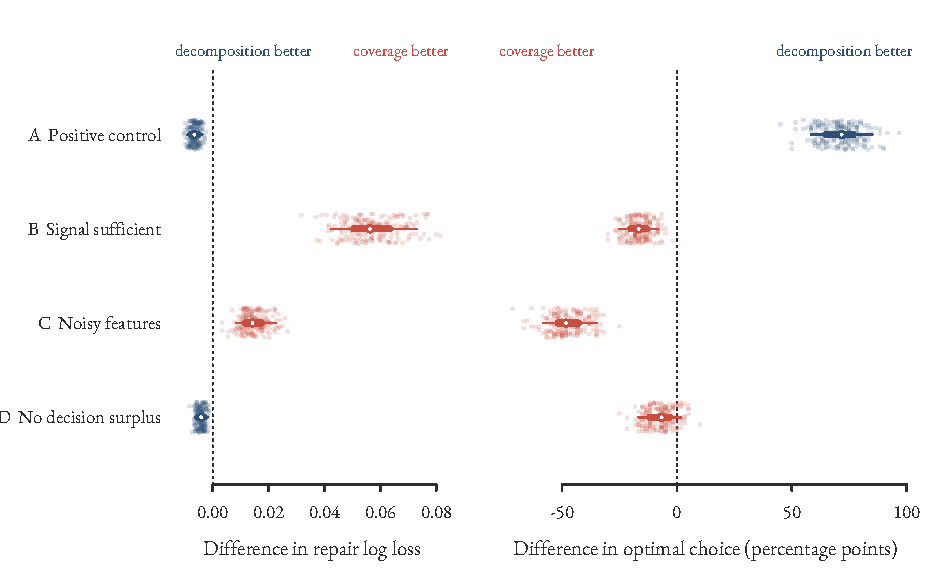
\includegraphics[width=\linewidth]{analysis/results/gelman_fake_data_paired_differences.pdf}};
\begin{scope}[x={(simulationplot.south east)},y={(simulationplot.north west)}]
  \node[anchor=north,font=\small\scshape] at (0.34,0.99) {Repair prediction};
  \node[anchor=north,font=\small\scshape] at (0.77,0.99) {Intervention choice};
\end{scope}
\end{tikzpicture}
\caption{Paired differences between the decomposition and conditional coverage across 200
constructed replications. Points show replications; thin and thick lines span the central 90
and 50 percent, and circles mark medians. Blue favours the decomposition and coral favours
conditional coverage, redundantly marked by position relative to zero. Each world is a
separate stress condition: A is a positive control, while B--D specify conditions under
which the decomposition can lose.}
\label{fig:fake-data}
\end{figure}

Figure~\ref{fig:fake-data} reports the audit. World A is a positive control: attribution and
uptake were built into the generating process and omitted from the comparator. Worlds B--D
carry the substantive burden.
Conditional coverage is sufficient in B. In C, route structure generates the data, but
noisy feature measurements make the decomposition choose the optimal intervention 47.23
percentage points less often. In D, it predicts repair better without improving
intervention choice. The decomposition earns its extra complexity only when its
distinctive features are causally important, measurable, and useful for prediction or
decisions.

Differences in final-accuracy loss are much smaller because initially correct answers
dominate that aggregate, which is why the article treats repair conditional on error and
harmful intervention as the more diagnostic quantities. The repair and regret comparisons
in each of the first three worlds have the same direction in all 200 replications; in the
fourth, decision regret is effectively tied. The reproducible R script and machine-readable
results accompany this resource.

\section{A crossed route-by-task design}

The worked example uses clinical questions. One item set asks for recommendations
recoverable from guidelines or institutional records. A paired set uses the same disease
area and answer format and requires a patient-specific lab value, observed sign, dose
calculation, or intervention-sensitive causal judgment. The prediction is a retrieval
gain on the record-recoverable set and little transfer to the patient-specific set unless
the needed measurement or tool route is supplied. Retrieval producing the same gain on
both sets would count against the proposed distinction between routes. The design parallels
validity argumentation in measurement: inferences from performance are licensed relative
to a purpose and tested by varying method while holding the target construct fixed
\citep{messick_1989_validity,kane2013validating}.

Matching the sets on difficulty cues isn't sufficient. An intervention that supplies a
missing lab value also makes the item easier, so a difficulty explanation and a route
explanation both predict a gain. Equating measured baseline accuracy weakens the simplest
difficulty account without eliminating differences in discrimination, ceiling structure,
response variance, latent subskills, or treatment-effect heterogeneity. Matching on noisy
estimates also invites regression to the mean. Use baseline performance as a covariate and
design diagnostic, not as evidence that difficulty has been removed.

The primary design is crossed rather than merely matched. Build item families in which the
relevant route can be supplied or withheld within closely related items, then cross route
availability against task requirement. Estimate the interaction in a hierarchical model
with varying effects for items, domains, prompt templates, and systems. Declare in advance
the smallest interaction that would matter, report its interval, and run reasonable
alternatives for item matching, scoring, and exclusion rather than relying on one sample.

In the single-pair implementation, the comparison uses two named chat arrangements that
differ only in whether retrieval over a fixed corpus is available, with the prompt template
held constant. The estimate is conditional on that pair; variation across model families
and deployment setups lies outside the estimand and belongs to a multi-system extension.
The population is a clinical item set split into record-recoverable and patient-specific
halves. Raters classify the items from their text without seeing system output, and the
classification is frozen before the first run.

The primary outcome is substantive correctness of the recommendation, scored blind, which
applies to both halves of the item set. Whether verbatim anchors resolve is secondary and
applies only within the record-dependent half. Making anchor resolution primary would
manufacture the interaction because patient-specific items have no corpus anchors to
resolve.

The worked prediction is that the retrieval gain on record-recoverable items exceeds the
gain on patient-specific items by at least ten percentage points. Ten is illustrative, not
derived. A defensible threshold needs a decision basis: the cost of a wrong recommendation,
the cost of retrieval latency, and what a deployment would do differently at nine points
rather than eleven. Fix the value before outcomes are observed so that the prediction can
fail.

The interval is interpreted against that threshold rather than zero. Concentration above
ten points supports the worked claim; concentration near zero or on the wrong side counts
against it. An interval extending from below zero to well above ten describes an
uninformative experiment, not evidence either way. The threshold isn't revised after the
effect becomes visible.

A stronger implementation crosses both interventions with both task types. Retrieval
should selectively help record-dependent items; a measurement tool should selectively help
items requiring measurement. This double dissociation tests the proposed route
carving, though a relevance-sensitive information account can predict the same qualitative
interaction.

\section{Checking-route independence}

Compare two checkers: one from the generator's lineage and the other trained and calibrated
on separate data and feedback. Give them the same candidate output and task evidence
supplied from outside the checkers. Match standalone accuracy, confidence, latency,
response format, and revision policy as closely as possible. Measure detection and
correction conditional on generator error, especially under perturbations expected to
produce common-mode failure.

Verify rather than assume the match. Use held-out calibration items to compare standalone
accuracy, confidence calibration, and latency, and route both checker outputs through the
same response format and revision policy. The primary cross-route quantity is conditional
error overlap: how often the checker repeats the generator's error when the generator is
wrong. Report it together with false interventions on generator outputs that were already
correct.

For this comparison, input coverage is measured before either checker produces a
task-specific signal. Checker outputs are downstream consequences of the architecture,
not part of baseline input coverage. If coverage is measured after a checker responds, the
predicted advantage is already a conditional-coverage effect.

The decomposition predicts an advantage for the checker with lower conditional error overlap.
Calibration history matters only insofar as it predicts that overlap; if admissible
perturbations produce no difference, the decomposition has no reason to privilege one history.
An input-coverage account predicts no advantage once externally supplied task information
and standalone accuracy are matched. A conditional-coverage account can predict one by
representing the joint error structure, but that prediction incorporates the relation that
checking-route independence names.

\section{A temporal test of live answerability}

Give two arrangements the same target information at the outset, one holding a frozen
pasted record and the other holding a live route to its source. In the update arm, correct
the source record and ask a follow-up whose answer turns on the correction. In the control
arm, leave the record unchanged. The live route should track the update in the first arm
and match the frozen copy in the second. Figure~\ref{fig:design-supplement} summarizes the
design.

\begin{figure}[H]
\centering
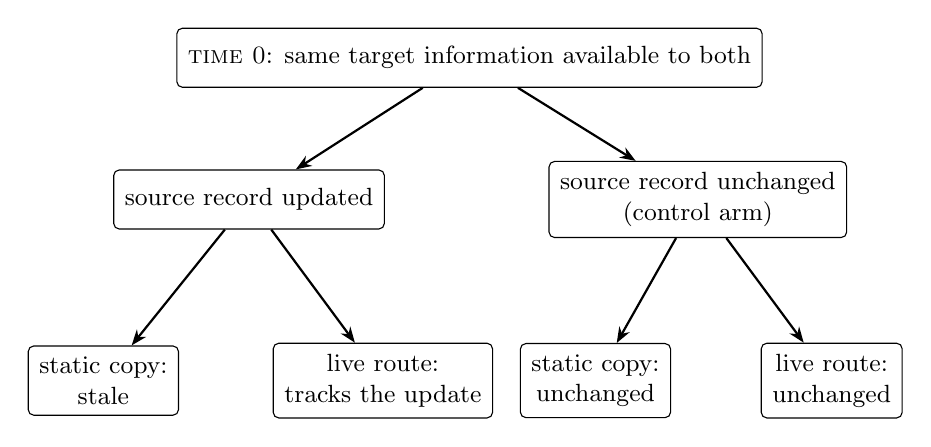
\begin{tikzpicture}
  \node[ttpbox] (t0) at (5,2.5) {\textsc{time 0}: same target information available to both};

  \node[ttpbox] (upd) at (2.2,0.7) {source record updated};
  \node[ttpbox] (ctl) at (7.9,0.7) {source record unchanged\\(control arm)};

  \node[ttpbox] (u1) at (0.35,-1.6) {static copy:\\stale};
  \node[ttpbox] (u2) at (3.9,-1.6)  {live route:\\tracks the update};
  \node[ttpbox] (c1) at (6.6,-1.6)  {static copy:\\unchanged};
  \node[ttpbox] (c2) at (9.6,-1.6)  {live route:\\unchanged};

  \draw[ttpar] (t0) -- (upd);
  \draw[ttpar] (t0) -- (ctl);
  \draw[ttpar] (upd) -- (u1);
  \draw[ttpar] (upd) -- (u2);
  \draw[ttpar] (ctl) -- (c1);
  \draw[ttpar] (ctl) -- (c2);
\end{tikzpicture}
\caption{A temporal test of live answerability. At time 0, both arrangements have the same
target information. In the update arm, the source record is corrected: the static copy
stays stale while the live route transmits the correction. In the control arm, neither
should change. No outcome magnitudes are implied.}\label{fig:design-supplement}
\end{figure}

A dynamic coverage account predicts the same pattern because the arrangements receive
different information at follow-up. The manipulation operationalizes live answerability and
isolates updateability from initial content equivalence; it doesn't adjudicate between the
decomposition and dynamic coverage.

\section{Manipulation checks and failure conditions}

Failure of a declared route-specific interaction or update effect counts against the
decomposition only after confirming that the focal route was invoked and that its output
reached production in time to affect the answer. A stale index, failed tool call, or ignored
checker signal shows that the intended manipulation wasn't instantiated. Once those checks
pass, failure of the declared contrast is evidence that the proposed route carving or
corrective feature has been misdescribed.

\printbibliography

\end{document}
